\chapter{协议设计}

\section{需求分析}

网络编程的服务端程序在大多数的情况下,并不只是与一个客户端进行通讯。在嵌入式行业中,设备通常被被要求至少同时需要与5-10个客户端同时通信,而对于嵌入式设备来说,其内部资源是非常有限的,我们本次使用select函数进行处理并发。本周要实现的是服务器能实现多个客户端的并发处理。即实现服务器在等待一个客户端发送下一个请求时,能够同时处理来自其它客户端的请求。

\section{并发客户端的设计方法和技术}

我们是利用select函数去实现并发客户端。函数  int select(int maxfd + 1,fd\_set *readset,fd\_set *writeset, fd\_set *exceptset,const struct timeval * timeout); 参数定义如表\ref{tb:select} 所示。

\begin{table}[htbp!]
    \centering
    \begin{tabular}{p{40pt}p{300pt}}
        \hline
    参数  & 描述  \\\hline

    参数一 & 最大的文件描述符 + 1。是一个整数值,是指集合中所有文件描述符的范围,即所有文件描述符的最大值加1。 \\

    参数二 & 用于检查可读性,是指向fd\_set结构的指针,这个集合中应该包括文件描述符,我们是要监视这些文件描述符的读变化的,即我们关心是否可以从这些文件中读取数据了,如果这个集合中有一个文件可读,select就会返回一个大于0的值,表示有文件可读,如果没有可读的文件,则根据timeout参数再判断是否超时,若超出timeout的时间,select返回0,若发生错误返回负值。可以传入NULL值,表示不关心任何文件的读变化。\\

    参数三 & 用于检查可写性,具体的解释同参数二一致。 \\

    参数四 & 用于检查文件错误异常,具体的解释同参数二一致。 \\

    参数五 & 用于指定select函数运行到此处时等待的时间。                                        \\\hline
    \end{tabular}
    \caption{select 函数参数描述} \label{tb:select}
    \end{table}
参数5可以使select处于三种状态
\begin{enumerate}
    \item 若将NULL以形参传入,即不传入时间结构,就是将select置于阻塞状态,一定等到监视文件描述符集合中某个文件描述符发生变化为止
    \item 若将时间值设为0秒0毫秒,就变成一个纯粹的非阻塞函数,不管文件描述符是否有变化,都立刻返回继续执行,文件无变化返回0,有变化返回一个正值;
    \item timeout的值大于0,这就是等待的超时时间,即select在timeout时间内阻塞,超时时间之内有事件到来就返回了,否则在超时后不管怎样一定返回,返回值同上述。
\end{enumerate}

\begin{figure}[htbp!]
    \centering
    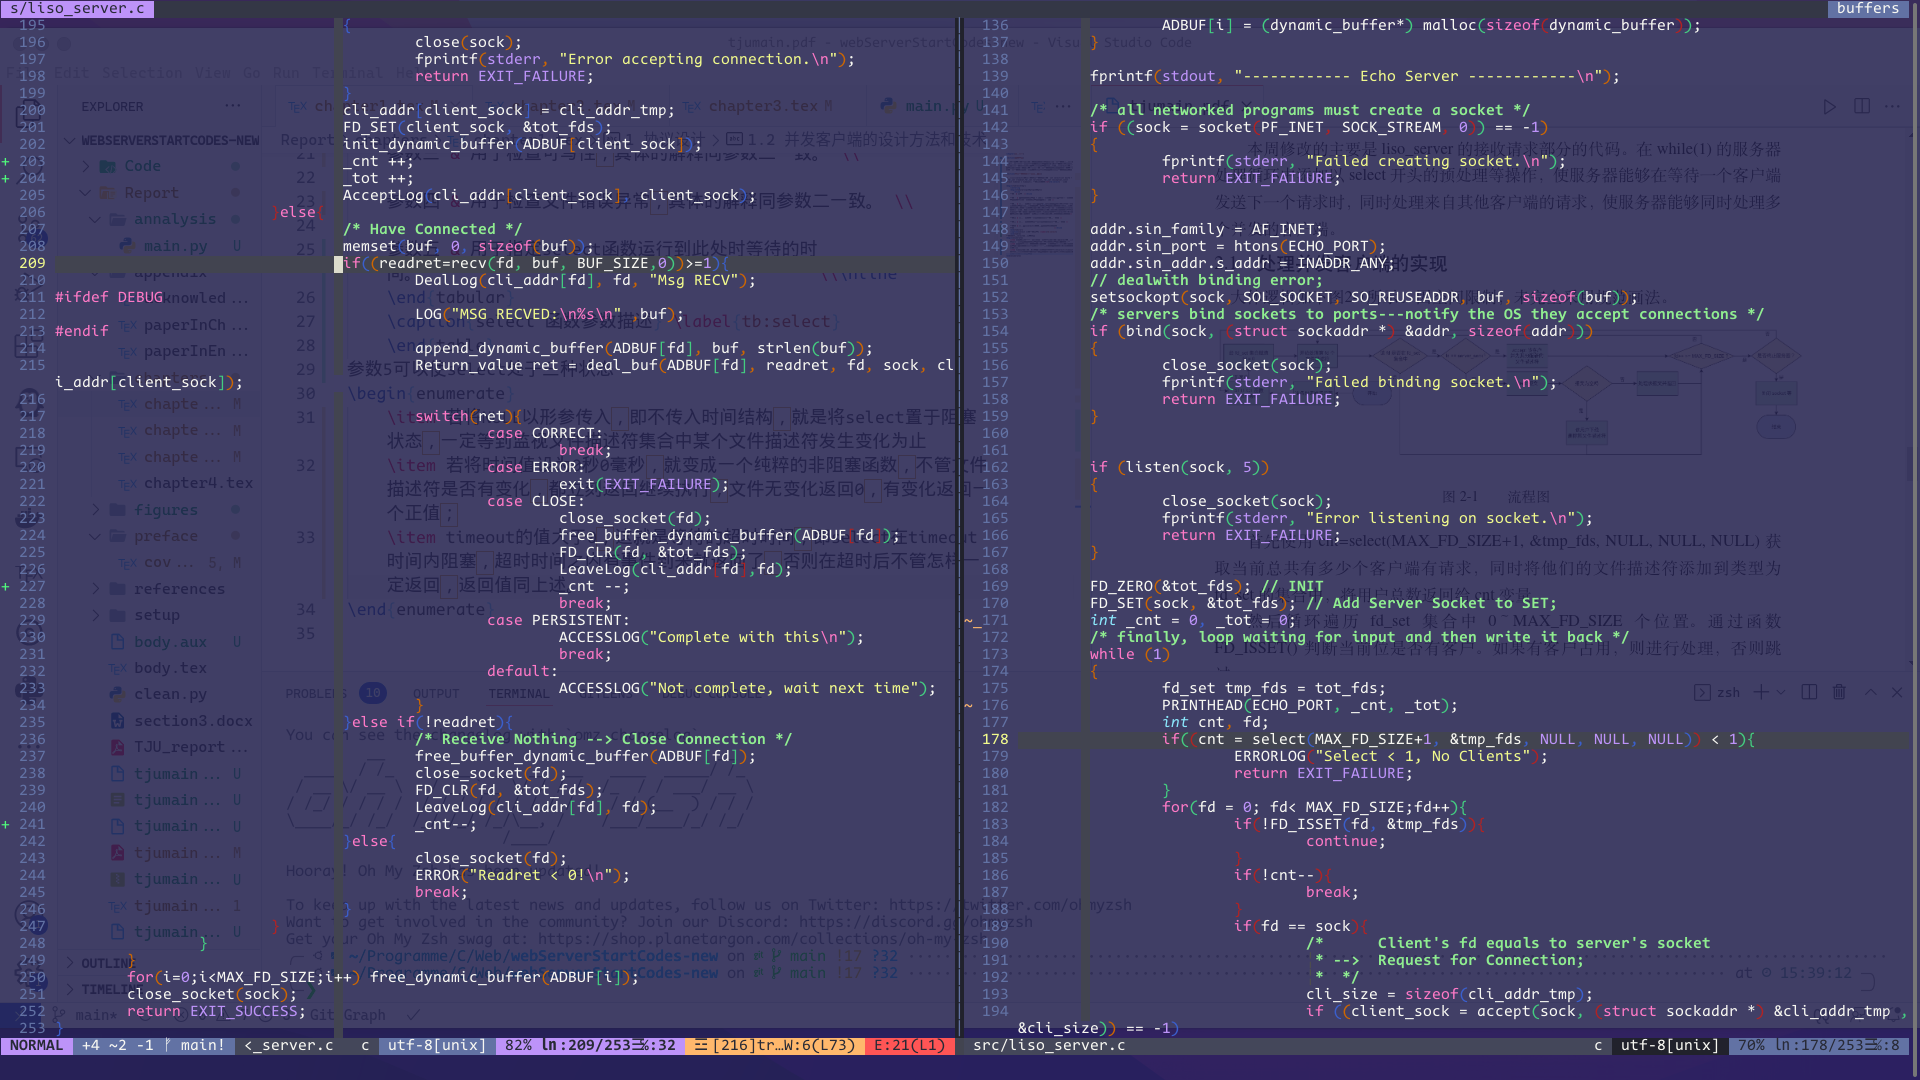
\includegraphics[width=5.5in]{liso_server_select.png}
    \caption{部分代码}\label{fig:SelectSource}
\end{figure}

部分代码如图\ref{fig:SelectSource} 所示,我们通过 select 阻塞后再遍历 fd 的集合进而对每个真实存在的用户进行服务。具体流程将在下一章具体展示。
